%%%%%%%%%%%%%%%%%%%%%%%%%%%%%%%%%%%%%%%%
% Classe do documento
%%%%%%%%%%%%%%%%%%%%%%%%%%%%%%%%%%%%%%%%

% Nós usamos a classe "unb-cic".  Deixe apenas uma das linhas
% abaixo não-comentada, dependendo se você for do bacharelado ou
% da licenciatura.

\documentclass[bacharelado]{unb-cic}
%\documentclass[licenciatura]{unb-cic}



%%%%%%%%%%%%%%%%%%%%%%%%%%%%%%%%%%%%%%%%
% Pacotes importados
%%%%%%%%%%%%%%%%%%%%%%%%%%%%%%%%%%%%%%%%

\usepackage[brazil,american]{babel}
\usepackage[T1]{fontenc}
\usepackage{indentfirst}
\usepackage{natbib}
\usepackage{xcolor,graphicx,url}
\usepackage{amsmath,amssymb,amsthm}		%Pacote da AMS para usar fórmulas
\usepackage[utf8]{inputenc}
\usepackage{listings}					%Formatação do código fonte
\usepackage{textcomp}


%%%%%%%%%%%%%%%%%%%%%%%%%%%%%%%%%%%%%%%%
% Cores dos links
%%%%%%%%%%%%%%%%%%%%%%%%%%%%%%%%%%%%%%%%

% Veja o arquivos cores.tex se quiser ver que outras cores estão
% pré-definidas.  Utilizando o comando \hypersetup abaixo nós
% evitamos aquelas caixas vermelhas feias em volta dos links.

%%%%%%%%%%%%%%%%%%%%%%%%%%%%%%%%%%%%%%%%
% Cores do estilo Tango
%%%%%%%%%%%%%%%%%%%%%%%%%%%%%%%%%%%%%%%%

\definecolor{LightButter}{rgb}{0.98,0.91,0.31}
\definecolor{LightOrange}{rgb}{0.98,0.68,0.24}
\definecolor{LightChocolate}{rgb}{0.91,0.72,0.43}
\definecolor{LightChameleon}{rgb}{0.54,0.88,0.20}
\definecolor{LightSkyBlue}{rgb}{0.45,0.62,0.81}
\definecolor{LightPlum}{rgb}{0.68,0.50,0.66}
\definecolor{LightScarletRed}{rgb}{0.93,0.16,0.16}
\definecolor{Butter}{rgb}{0.93,0.86,0.25}
\definecolor{Orange}{rgb}{0.96,0.47,0.00}
\definecolor{Chocolate}{rgb}{0.75,0.49,0.07}
\definecolor{Chameleon}{rgb}{0.45,0.82,0.09}
\definecolor{SkyBlue}{rgb}{0.20,0.39,0.64}
\definecolor{Plum}{rgb}{0.46,0.31,0.48}
\definecolor{ScarletRed}{rgb}{0.80,0.00,0.00}
\definecolor{DarkButter}{rgb}{0.77,0.62,0.00}
\definecolor{DarkOrange}{rgb}{0.80,0.36,0.00}
\definecolor{DarkChocolate}{rgb}{0.56,0.35,0.01}
\definecolor{DarkChameleon}{rgb}{0.30,0.60,0.02}
\definecolor{DarkSkyBlue}{rgb}{0.12,0.29,0.53}
\definecolor{DarkPlum}{rgb}{0.36,0.21,0.40}
\definecolor{DarkScarletRed}{rgb}{0.64,0.00,0.00}
\definecolor{Aluminium1}{rgb}{0.93,0.93,0.92}
\definecolor{Aluminium2}{rgb}{0.82,0.84,0.81}
\definecolor{Aluminium3}{rgb}{0.73,0.74,0.71}
\definecolor{Aluminium4}{rgb}{0.53,0.54,0.52}
\definecolor{Aluminium5}{rgb}{0.33,0.34,0.32}
\definecolor{Aluminium6}{rgb}{0.18,0.20,0.21}

\hypersetup{
  colorlinks=true,
  linkcolor=DarkScarletRed,
  citecolor=DarkScarletRed,
  filecolor=DarkScarletRed,
  urlcolor= DarkScarletRed
}

%%%%%%%%%%%%%%%%%%%%%%%%%%%%%%%%%%%%%%%%
% Informações sobre a monografia
%%%%%%%%%%%%%%%%%%%%%%%%%%%%%%%%%%%%%%%%

\title{Confiabilidade em Sistemas Multiagentes}

\orientador{\prof Célia Ralha}{CIC/UnB}
\coordenador{\prof Marcus Vinícus Lamar}{CIC/UnB}
\diamesano{12}{dezembro}{2012}

\membrobanca{\prof Genaína Nunes}{CIC/UnB}
\membrobanca{\prof Professor II}{CIC/UnB}

\autor{João Paulo de Freitas}{Matos}
\CDU{004.4}

\palavraschave{Confiabilidade, Sistemas Multiagentes}
\keywords{Reliability, Multiagent systems}

%%%%%%%%%%%%%%%%%%%%%%%%%%%%%%%%%%%%%%%%
% Texto
%%%%%%%%%%%%%%%%%%%%%%%%%%%%%%%%%%%%%%%%

\begin{document}
  \maketitle
  \pretextual

  \begin{dedicatoria}
  Dedico a....
  \end{dedicatoria}

  \begin{agradecimentos}
  Agradeço a....
  \end{agradecimentos}

  \begin{resumo}
  A ciência...
  \end{resumo}

  \selectlanguage{american}
  \begin{abstract}
  The science...
  \end{abstract}
  \selectlanguage{brazil}

  \tableofcontents
  \listoffigures
  \listoftables

  \textual
  \chapter{Introdução}

Cada pessoa possui uma forma preferencial de absorção do conhecimento. Seja por imagens, textos, teoria ou prática, durante uma situação de aprendizagem todos tendem a receber e processar melhor as informações que são recebidas de certa maneira, em detrimento a outras. Essa forma de recepção do conhecimento é nomeada estilo de aprendizagem.
 
O acesso à recursos tecnológicos que, outrora caros e difíceis, tornaram-se presentes no cotidiano de muitas pessoas devido a facilidade de aquisição. Dessa forma, a viabilidade do aprendizado por meio do computador aumentou e começa a modificar o paradigma do professor detentor do conhecimento e o único responśavel pela sua transmissão.

Em um ambiente escolar a forma didática escolhida por um docente pode afetar o desempenho dos seus alunos, visto que a forma de transmissão do conhecimento escolhida pode desprivilegiar alguns estudantes. A situação ideal requer a existência de uma personalização do ensino para cada estudante, considerando as características inerentes à sua cognição. Inspirado por esse ideal, algumas ferramentas no âmbito da computação pretendem planejam o ensino personalizado para cada estudante de acordo com o seu perfil de utilização, primeiramente pelo grande acesso da sociedade à computadores e também devido à diversos estudos relacionados na área de educação.

Conhecer os fatores relacionados ao processo de aprendizagem exige que as ferramentas computacionais aplicadas ao ensino consigam determinar eficientemente os estilos de aprendizagem. Assim, a complexidade das aplicações aumenta devido às abordagens que serão empregadas, bem como a exigência de processamento que podem exigir.

Algumas abordagens visam diminuir essa complexidade, permitindo a representação aproximada das características dos alunos em ambientes computacionais, de forma que possam coexistir em um mesmo ambiente vários modelos de estudantes. Por exemplo, o modelo do estudante elaborado na forma multidimensional a partir dos universos cognitivo, metacognitivo e afetivo.

Somado à isso, técnicas de computação distribuída são projetadas para rodar de forma descentralizada, com componentes e serviços rodando em diversos lugares distintos e comunicando-se uma com as outras através de mensagens. A arquitetura dessas aplicações é projetada objetivando o alto paralelismo, exibilidade, interoperabilidade, dentre outros aspectos.

Portanto, determinar o estilo de aprendizagem mostra-se uma estratégia fundamental para que a transmissão de informações e vivências entre alunos e professores torne-se mais eficaz e perceptível, promovendo a criação de informações cada vez mais relevantes para o planejamento, acompanhamento e avaliação dos aprendizes.


\section{Problema}
Os ambientes educacionais de aprendizagem não possuem uma arquitetura apropriada para a inferência de modelos multidimensionais, pois a abordagem baseada em cliente-servidor não é razoável para representação de perfis de alunos no ambiente.

\section{Objetivos}
Tendo em vista o cenário atual apresentado, o presente trabalho tem como objetivo definir uma arquitetura distribuída na Web para auxiliar o processo de ensino-aprendizagem por meio da abordagem de Sistema multiagente (SMA), criando insumos para auxiliar o docente na adoção da melhor estratégia didática de ensino.

Esta abordagem permitirá a construção e manutenção de um modelo multidimensional do estudante, a partir do qual os estilos de aprendizagem desse estudante poderão ser identificados. A abordagem de sistemas multiagentes permite a decomposição do problema na modelagem multidimensional em vários subproblemas menores, sendo capaz de diminuir a complexidade da resolucão. Além disso características inerentes aos agentes, como a habilidade social dos agentes, podem permitir a interação com outros modelos de alunos visando comparações e validações do modelo.

Em corroboração ao objetivo do trabalho, a informação do estilo de aprendizagem ao docente pode permitir a correta orientação da sua didática em sala de aula, melhorando qualitativamente o ensino aos seus alunos.

Especificamente, os objetivos deste trabalho são:
\begin{itemize}
 	\item Projeto da arquitetura geral de um sistema multiagente, utilizando-se de uma metodologia apropriada;
	\item Definir e implementar a arquitetura geral da solução, incluindo os agentes assistentes de cognição, metacognição e afetivo;
	\item Propor uma interface do agente assistente de cognição com os atores externos do sistema: Docente e Estudante;
\end{itemize}

\section{Metodologia}

A metodologia de realização deste trabalho é constituída da revisão bibliográfica, modelagem da arquitetura, implementação e testes em laboratório da solução. A primeira etapa consistiu do estudo dos conceitos de Informática na Educação, Sistemas Multiagentes e levantamentos de uso de SMA em contextos pegagógicos. Este estudo foi importante para a orientação do desenvolvimento embasado na teoria e a comparação das ferramentas existentes com a solução proposta.

Em seguida, foi realizado o levantamento e estudo de metodologias aproriadas para modelagem de SMA existentes para a modelagem e construção da solução. Essas metodologias foram comparadas e uma delas escolhida para o desenvolvimento da aplicação. Após a escolha da metodologia de desenvolvimento, foi feita a modelagem do SMA com a metodologia em questão.

O desenvolvimento da aplicação multiagente foi feito com o~\emph{framework}~\emph{JADE}. Que é completamente desenvolvido na linguagem~\emph{JAVA} e simplifica a implementação de Sistemas Multiagentes (SMA) que cumprem as especificações FIPA. 

Em seguida, foi necessário a escolha de uma ferramenta para desenvolvimento da interface web e a sua integração com o sistema multiagente. Baseado nos estudos feitos, o~\emph{framework JBoss Seam} mostrou-se mais viável visto que facilita a construção de aplicações dinâmicas para a internet de forma simples e ágil.

Por fim, foram realizados testes em laboratório da solução proposta. Foram definidos cenários que simulavam o uso da aplicação por meio dos perfis de Aluno e Docente.

\section{Estrutura do Trabalho}
A divisão de capítulos foi feita da seguinte forma:
\begin{itemize}
	\item Capítulo 2: Apresenta uma breve visão sobre as áreas de estudo envolvidas neste trabalho: Informática na Educação, Sistema Multiagente. Além disso, apresenta algumas ferramentas e tecnologias utilizadas, bem como os trabalhos correlatos e um comparativo.
	\item Capítulo 3: Contém a proposta de solução composta pela metodologia, modelagem da arquitetura e implementação.
	\item Capítulo 4: Exibe os testes realizados em laboratório por meio dos perfis dos usuários: Aluno e Docente.
	\item Capítulo 5: Apresenta algumas conclusões e abre perspectivas para trabalhos futuros.
\end{itemize}

  \chapter{Fundamentos básicos}

Este capitulo apresenta os principais conceitos e definições necessários para o entendimento deste trabalho. A seção 2.1 apresenta alguns conceitos básicos em~\emph{Unified Modeling Language} (UML), que são necessários para o entendimento da modelagem deste trabalho.
A seção 2.2 disserta sobre conceitos a respeito da informática na educação.
A seção 2.3 aborda a teoria sobre Sistemas Multiagentes necessária para este trabalho.
A seção 2.4 contém a metodologia~\emph{Multiagent System Engineering}, desenvolvida para a criação de Sistemas Multiagentes
A seção 2.5 e 2.6 abordam o funcionamento dos frameworks JADE e Jboss Seam, respectivamente.
Por fim, a seção 2.7 detalha alguns trabalhos correlatos.

\section{Unified Modeling Language}

A Linguagem Unificada de Modelagem,~\emph{Unified Modeling Language} (UML) é uma linguagem visual que foi desenvolvida para a representação do software por meio de imagens, objetivando o entendimento dos artefatos de forma rápida e clara e resultando em uma semântica para o projeto em questão. De acordo com~\cite{fowler04} o UML faz parte de uma família de notações gráficas que ajudam na descrição e concepção de sistemas de software, principalmente em sistemas concebidos utilizando o paradigma da orientação à objetos (OO).

O UML é um padrão não proprietário, controlado pelo consórcio~\emph{Object Management Group}~\cite{omg20}. Seu nascimento é datado em 1997~\cite{fowler04}, surgindo a partir da união de diversas linguagens e ferramentas de surgiram na década de 80 e 90.
A linguagem ajuda o entendimento de como o software foi projetado, como ocorre a comunicação entre seus objetos, como suas classes são organizadas, quais são os atores que são envolvidos na utilização do software, dentre outras possibilidades de representação.

Em~\cite{fowler04}, é possível separar o uso do UML de três formas distintas, diferindo entre as modelagens utilizadas e o objetivo de uso. As três formas são: Rascunho, planta de software e como linguagem de programação. 

A utilização como rascunho é utilizada para facilitar a comunicação entre as pessoas envolvidas no projeto, sejam desenvolvedores discutindo funcionalidades do software ou gestores explicando funcionalidades em alto nível. O objetivo neste uso é a comunicação de alguns aspectos do sistema de forma rápida, sem a necessidade de formalizar artefatos para o projeto.

A utilização do UML como planta de software são documentos detalhados que são criados para documentação do software, sendo divida em duas sub-categorias: Engenharia reversa e engenharia avante. Na engenharia reversa, os diagramas são gerados a partir de uma ferramenta que faz a leitura do código fonte e gera os diagramas desejados, que são utilizados para auxiliar o leitor no entendimento do sistema. Na engenharia avante, a idéia é modelar o sistema detalhadamente antes de qualquer desenvolvimento, prevendo quais serão os módulos do sistema, bem como a sua a comunicação.

No uso como linguagem de programação, o UML é utilizado para geração de código executável por ferramentas avançadas de modelagem. Esse modo requer a modelagem de estado e comportamento do sistema, para fins de detalhar todo o comportamento e lógica do sistema em código.

\subsection{Diagramas UML}

O UML 2 descreve 13 tipos de diagramas que podem ser categorizados por estruturais e comportamentais. A imagem~\ref{fig:categorias-diagramas} ilustra essa categorização de diagramas.

\begin{figure}
	\centering
	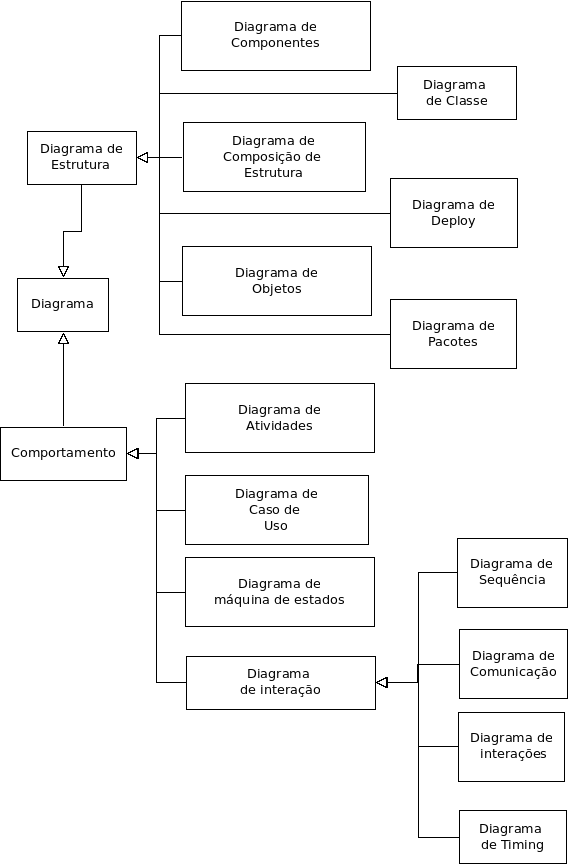
\includegraphics[scale=0.75]{images/categorias-diagramas.png}
	\caption{Diagramas categorizados por Estrutura e Comportamento. Fonte~\cite{fowler04}.}
	\label{fig:categorias-diagramas}
\end{figure}

Apesar da grande quantidade diagramas envolvidos no UML, nem todos os processos de desenvolvimentos de software utilizam todos eles. A maioria das pessoas utiliza-se de um conjunto de poucos diagramas para modelagem do sistema. Nas próximas subseções, serão detalhados apenas os seguintes diagramas, que são necessários para o entendimento deste trabalho:

\begin{itemize}
	\item Diagrama de Caso de uso
	\item Diagrama de sequência
\end{itemize}

\subsubsection{Diagrama de Caso de Uso}
Casos de uso são relatos textuais que são utilizados para descobrir e descrever os requisitos do sistema. Consiste da descrição de como um ator utiliza uma funcionalidade do sistema para atingir algum objetivo relacionado. De acordo com~\cite{larman08}, os casos de uso devem ser prioritariamente desenvolvidos de forma textual e o seu respectivo diagrama deve ser desenvolvido de forma secundária, somente para ilustrar o relato textual.

Um dos objetivos do caso de uso é a facilidade do levantamento dos requisitos, tanto para os analistas de um sistema, quanto para os clientes envolvidos. A definição de uma modelagem em comum facilidade entre as partes faz do caso de uso uma boa maneira de simplificar o entendimento do comportamento do sistema~\cite{larman08}, bem como envolver todos as partes interessadas do sistema(~\emph{stakeholders}) na construção do mesmo. De acordo com~\cite{cockburn01}, o caso de uso é um contrato de como será o comportamento do sistema. Este contrato será feito por meio dos atores que existirão, da sua interação com o sistema, bem como os cenários existentes.

Duas definições fazem-se necessárias para o entendimento do caso de uso. A primeira delas é o "Ator" do caso de uso. Ele é um objeto com um comportamento definido no sistema. É possível definir o ator como uma pessoa, organização ou mesmo o próprio sistema (quando utiliza serviços do próprio sistema), desde que tenham sempre um papel relacionado. Existem três tipos de atores relacionados ao sistema:
\begin{itemize}
	\item Ator Principal: Seus objetivos são satisfeitos por meio da utilização do sistema.
	\item Ator de Suporte: Fornece algum serviço para o sistema.
	\item Ator de Bastidor: Expressa algum interesse pelo comportamento do caso de uso.
\end{itemize}

A segunda definição envolvida é a de cenário. Um cenário é uma sequência de interações entre os atores e o sistema. Os cenários são separados por ações de interesses de atores. Logo o caso de uso pode ser considerado como um conjunto de cenários de interações de atores com o sistema.

Dessa forma, o caso de uso deve deixar claro os requisitos funcionais do sistema, bem como o seu comportamento. Existem três formas de se escrever um caso de uso, diferindo em seu nível de formalidade e formatos: Resumido, informal e completo. Este trabalho usará o nível de caso de uso completo, devido ao fato de ser estruturado e mostrar mais detalhes. Os casos de uso são estruturados de diversas formas de acordo com a literatura, sendo a mais famosa~\cite{larman08} a estrutura utilizada por Alistar Cockburn~\cite{cockburn01} e detalhada na tabela~\ref{tabela:topicos_uc}

\begin{table}
	\caption{Estruturação Detalhada de Caso de Uso}
	\begin{tabular}{|p{5cm} | p{9cm}|}
		\hline
		\textbf{Seção do Caso de Uso}	& \textbf{Significado} \\
		\hline
		Nome do Caso de Uso 	& Nome do caso de uso, iniciando-se com um verbo  \\
		\hline
		Escopo	& Escopo descrito pelo caso de uso \\
		\hline
		Nível	& Podem ser níveis de objetivo de usuário (quando descrevem os cenários para atingir o objetivo do usuário) ou nível de subfunção (subpassos para dar suporte a um objetivo de usuário) \\
		\hline
		Ator Principal	& O ator que procura os serviços para atingir seus objetivos  \\
		\hline
		Interessados e Interesses	& Significado  \\
		\hline
		Pré-Condições	& Condições que antecedem o caso de uso e são necessárias para atingir os objetivos \\
		\hline
		Garantia de Sucesso	& Objetos que podem ser analisados após a execução do caso de uso a fim de validar a correta execução do sistema  \\
		\hline
		Cenário de Sucesso Principal	& Chamado também de fluxo básico, este cenário descreve o fluxo principal do sistema que satisfaz os interesses dos interessados.  \\
		\hline
		Extensões	& Chamado também de fluxos alternativos, são fluxos auxiliares ou cenários de erros que são relacionados ao cenário de sucesso principal \\
		\hline
		Requisitos Especiais	& Registram requisitos não funcionais do sistema e que estão relacionados com o caso de uso \\
		\hline
		Lista de Variantes Tecnologias de Dados	& Listagem de dificuldades técnicas, desafios técnicos que valem a pena registrar no caso de uso \\
		\hline
		Frequência de ocorrência	& Frequência de ocorrência deste caso de uso \\
		\hline
	\end{tabular}
	\label{tabela:topicos_uc}
\end{table}

A diagramação do caso de uso por UML é uma forma de representação do sistema, mostrando fronteiras do sistema, comunicação e comportamento entre os atores. A figura~\ref{fig:diagrama-uml} mostra a sugestão de diagramação do caso de uso, propondo forma de representação de atores, casos de uso e atores auxiliares.

\begin{figure}
	\centering
	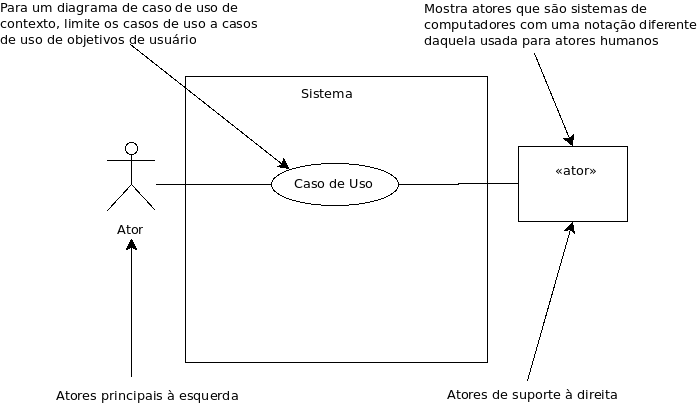
\includegraphics[scale=0.75]{images/exemplo-uml.png}
	\caption{Sugestões de notação de caso de uso proposto por ~\cite{larman08}}
	\label{fig:diagrama-uml}
\end{figure}

\subsubsection{Diagrama de Sequência}
O Diagrama de Sequência é um documento criado que ilustra os eventos do sistema de forma sequencial dentro de um caso de uso, mostrando a interação de atores externos ao sistema e os eventos que eles geram durante essa interação. A UML possui uma notação para o DSS, onde são representados as interações entre os atores e os eventos gerados por eles. 

Neste diagrama, são representados para cada cenário do caso de uso os eventos que os atores geram, bem como a ordem da sua interação. No diagrama são representados na parte superior (com a mesma notação do diagrama de caso de uso). Abaixo dos atores é representada a linha de tempo, crescendo de cima para baixo. Na linha de tempo, os eventos ocorrem na forma de interação entre os atores e de forma a seguir a mesma ordem os eventos no cenário. Os eventos devem sempre iniciar com um verbo podendo ser seguidos de um substantivo. Eles devem sempre ser expressos em níveis genéricos verbais, nunca detalhando a funcionalidade do sistema.

Durante a interação do ator com o sistema, eventos de sistema são gerados e iniciam toda a execução do cenário do caso de uso, ou operação do sistema. A execução dos eventos ocorre até o último evento gerado na linha do tempo do diagrama. A imagem~\ref{fig:diagrama-sequencia} ilustra a notação de diagramas de sequência com todos os pontos que foram até agora expostos.

\begin{figure}
	\centering
	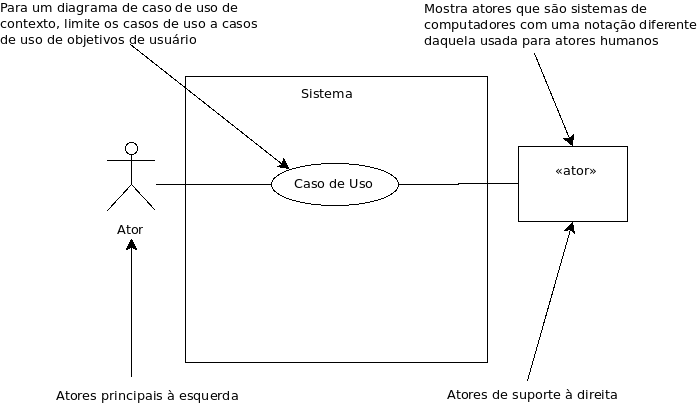
\includegraphics[scale=0.75]{images/exemplo-uml.png}
	\caption{Sugestões de notação de diagrama de sequência proposto por ~\cite{larman08}}
	\label{fig:diagrama-sequencia}
\end{figure}

A importância no desenho de um diagrama de sequência está no fato de saber exatamente os eventos externos gerados pela interação de atores externos, pois assim é possível ter uma análise comportamental do sistema com base nesses eventos. Neste nível de análise, o comportamento do sistema é uma descrição do que um sistema faz, sem explicar como o faz~\ref{larman08}.

O diagrama de sequência necessita estar sempre relacionado com o caso de uso, primeiramente pelo fato de sempre descrever um cenário de caso de uso, mas também pelo fato de o caso de uso conter todos os detalhes do cenário. O diagrama de sequência irá apenas deixar claro a interação entre os atores e os eventos derivados dessa interação.

\section{Informática na Educação}

\section{Sistemas Multiagentes}

\subsection{Inteligência artificial}

Antes de explicarmos o conceito de sistemas multiagentes (SMA), é necessário mostrar conceitos que são base para o entendimento de SMA. Inicia-se apresentando alguns conceitos de Inteligencia Artificial (IA). De acordo com~\cite{poole98} identificamos que a definição de IA pode variar em duas dimensões principais. Usando a definição de sistemas computacionais que agem racionalmente temos:

\begin{quote}
\emph{Computational Intelligence is the study of the design of intelligent agents.}
\end{quote}

Nessa definição, é importante ressaltar que o agente é uma entidade que atua racionalmente, esperando-se que essa racionalidade e outras características o diferencie de simples programas.

Com o crescimento dos estudos relacionado a este campo, a inteligência artificial ganhou várias áreas de atuação e resolução de problemas no nosso cotidiano. Um dos problemas é a necessidade de executar aplicações que resolvem problemas de alta complexidade. Essas aplicações podem exigir um hardware muito caro para a execução, ou então pode-se usar a abordagem de distribuí-la em vários computadores que dividem a sua execução. É justamente onde entra a inteligência artificial distribuída: São sistemas que são compostos por vários agentes coletivos, ou seja, distribuem o trabalho uns com os outros. Cada agente pode possuir uma capacidade diferente, sendo possível realizar a tarefa de modo paralelo. 

\subsection{Agente}

De acordo com~\cite{novig95}, agentes são entidades (reais ou virtuais) que funcionam de forma autônoma em um ambiente, ou seja, não necessitam de intervenção humana para realizar processamento. Esse ambiente de funcionamento do agente geralmente contém vários outros agentes e é possível a comunicação entre eles através do ambiente por meio de troca de mensagens.

Em geral o funcionamento de agentes acontece de forma a perceberem o ambiente em que estão por meio de sensores, fazem análises com base nessa interação inicial e por fim podem agir sobre o ambiente de forma a modifica-lo por meio de efetuadores. A figura~\ref{fig:agente-basico} apresenta um resumo do que foi dito.

\begin{figure}
	\centering
	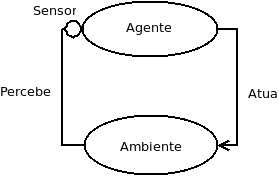
\includegraphics[scale=0.75]{images/agente-basico.png}
	\caption{Esquematização do funcionamento básico de um agente em um ambiente.}
	\label{fig:agente-basico}
\end{figure}

Agentes racionais seguem o princípio de racionalidade básico: sempre objetivam suas ações pela escolha da melhor ação possível segundo seus conhecimentos. Logo é possível inferir que a ação de um agente nem sempre alcança o máximo desempenho, sendo desempenho o parâmetro definido para medir o grau de sucesso da ação de um agente com base nos seus objetivos.

Como dito anteriormente, agentes estão presentes em um ambiente. O agente não tem controle total do ambiente, ele pode no máximo influenciá-lo com a sua atuação. Podemos separar ambientes em classes: Software, Físico e Relidade virtual (simulação de ambientes reais em software). De acordo com~\cite{wooldridge04} temos, em geral, ambientes tem propriedades inerentes que dizem respeito ao seu funcionamento:

\begin{itemize}
	\item Observável: Neste tipo de ambiente, os sensores dos agentes conseguem ter percepção completa do ambiente. Por exemplo, um sensor de movimento consegue ter visão total em um ambiente aberto.
	\item Determinística: O próximo estado do ambiente é sempre conhecido dado o estado atual do ambiente e as ações dos agentes. O oposto do ambiente determinístico é o estocástico, quando não temos certeza do estado do ambiente. Por exemplo, agentes dependentes de eventos climáticos.
	\item Episódico: A experiência do agente é dividida em episódios, onde cada episódio é a percepção do agente e a sua ação.
	\item Sequêncial: A ação tomada pelo agente pode afetar o estado do ambiente e ocasionar na mudança de estado
	\item Estático: O ambiente não é alterado enquanto um agente escolhe uma ação.
	\item Discreto: Existe um número definido de ações e percepções do agente para o ambiente em cada turno.
	\item Contínuo: As percepções e ações de um agente modificam-se em um espectro contínuo de valores. Por exemplo, temperatura de um sensor muda de forma contínua.
\end{itemize}

Na tabela~\ref{lista_agentes} mostramos alguns exemplos de agentes, apresentando as suas características já discutidas nesse trabalho.

\begin{table}
	\caption{Listagem de sistemas multiagentes com propriedades de medida de performance, ambiente, atuadores e sensores}
	\begin{tabular}{|p{3cm} | p{3cm} | p{2cm}| p{3cm} | p{3cm} |}
		\hline
		\textbf{Tipo de agente}	& \textbf{Medida de performance} & \textbf{Ambiente} & \textbf{Atuadores}  & \textbf{Sensores}	\\
		\hline
		Sensores de estacionamento	& Avarias no veículo & Carro e garagens & Freio do carro, controle de velocidade & Sensor de proximidade	\\
		\hline
		Jogos com oponente computador	& Quantidade de vitórias &	Software & Realizar jogada & Percepção do tabuleiro	\\
		\hline
		Agentes hospitalares		& Saúde do paciente & Paciente, ambiente médico & Diagnósticos & Entrada de sintomas do paciente	\\
		\hline
	\end{tabular}
	\label{lista_agentes}
\end{table}
 
A primeira linha da tabela~\ref{lista_agentes} é apresentado um exemplo de um agente atuando em um veículo como um sensor de estacionamento. Responsável por auxiliar o motorista no ato de estacionar o carro, o seu ambiente é da classe físico (considerando o carro e o ambiente onde está o carro). Seu sensor de proximidade é a percepção do ambiente e caso detecte que está próximo de um obstáculo pode atuar nos freios dos carros diminuindo a velocidade e evitando colisões. Avarias no carro podem indicar um mal funcionamento do sensor.

A segunda linha da tabela é apresentado u exemplo de agente atuando em um jogo qualquer. Esse ambiente é dito dinâmico, pois a cada jogada de um oponente (real ou não), o agente irá analisar a jogada feita pelo seu oponente, irá calcular sua próxima jogada e irá realizá-la. O objetivo principal do agente é a vitória. O ambiente que o agente atua é um software e o seu atuador é um algum mecanismo que permite que ele realize a jogada. O sensor é o mecanismo no qual o agente irá perceber a jogada realizada pelo oponente.

Por fim, última linha da tabela~\ref{lista_agentes} expõe um exemplo de um agente médico atuando em um ambiente estático um paciente. Esse ambiente é dito estático por que não será alterado pelo agente nesse exemplo, mas podendo ser diferente dependendo da aplicação. O objetivo principal é monitorar a saúde do paciênte, logo a medida de performance será a aproximação ou não do diagnóstico médico. Seu atuador não será diretamente no ambiente (corpo humano), será na forma de relatórios médicos e seus sensores podem variar de acordo com a doença a ser monitorada.

Conforme podemos encontrar em~\cite{wooldridge04}, podemos definir algumas noções gerais de agentes. A primeira, chamada de noção fraca, contém a maior parte dos agentes. Ela compreende os aspectos de \emph{reatividade}, \emph{proatividade} e \emph{habilidade social}. O conceito de reatividade  está ligado com o agente perceber o ambiente e reagir. Proatividade é a característica do agente tomar a iniciativa e agir sem a necessidade de nenhum estímulo. Habilidade social é a capacidade de interação com outros agentes.

Já a noção forte de agente envolve os seguintes aspectos: , veracidade, benevolência
\begin{itemize}
	\item Mobilidade: O Agente deve pode mover-se no ambiente, por exemplo, em uma rede.
	\item Veracidade: Agente não comunica informações falsas.
	\item Benevolência: Agente ajudará os outros.
	\item Racionalidade: O agente não irá agir de forma a impedir a realização de seus objetivos.
	\item Cooperação: O agente coopera com o usuário.
\end{itemize}

\subsection{Arquitetura de agentes}

A arquitetura de agentes varia de acordo com a complexidade da sua autonomia, ou seja, com a capacidade de reagir aos estímulos do ambiente. Conforme verificado no livro de ~\cite{novig95}, os tipos de arquitetura são: orientadas à tabela, reflexiva simples, reflexiva baseado em modelo, baseada em objetivo, baseada em utilidade.

A primeira arquitetura a ser explorada é o agente orientado à tabelas. Todas as ações dos agentes dessa arquitetura são conhecidas e estão gravadas em uma tabela. Assim, quando o agente receber o estímulo ele já terá a ação a ser tomada previamente gravada em sua memória. Logo para construir esse tipo de agente, fica claro que além de saber todas percepções possívels, será necessário definir ações apropriadas para todas. Isso levará a tabelas muito complexas e o tamanho pode facilmente passar a ordem de milhões dependendo do número de entradas.

A arquitetura reflexiva simples é um dos tipos mais simples de agente. Nele, o agente seleciona a ação com base unicamente na percepção atual, desconsiderando assim uma grande tabela de decisões. A decisão é tomada com base de regras condição-ação: Se uma condição ocorrer, uma ação será tomada. Por exemplo, vamos supor um agente médico que determina o diagnóstico de uma doença no paciente caso exista alguma anomalia no organismo (Por exemplo, paciente com febre). Uma condição-ação poderia ser:

if anomalia-organismo then diagnóstico-médico

Esse tipo de agente é bastante simples, o que é uma vantagem comparado à arquitetura de tabela. Porém, essa abordagem requer um ambiente totalmente observável, visto que esse tipo de agente possui uma inteligência bastante limitada. No exemplo do agente médico existem diversas maneiras de se detectar uma anomalia no organismo do paciente, seria necessário conhecer todas as formas para usarmos uma abordagem reativa simples.

A arquitetura reflexiva baseada em modelos funciona de maneira similar a anterior. Nessa abordagem, é levado em conta a parte do ambiente que não é visível neste momento. E para saber o ``momento atual'' de um agente, é necessário guardar a informação de estado consigo. Para atualizar o estado do agente, é necessário conhecer como o mundo desenvolve-se independente do agente (no caso do exemplo, como o organismo funciona) e é necessário saber as ações dos agentes no ambiente. Esses dois conhecimentos do ambiente são chamados de \textbf{modelo do mundo}. O agente que usa esse tipo de abordagem é chamado de agente baseado em modelo.

Na arquitetura reflexiva baseada em objetivo, as ações do agente são tomadas apenas se o aproximam de alcançar um objetivo. Para isso, será necessário algo além do estado atual do ambiente: Será necessário informações do objetivo a ser atingido. Assim o agente pode combinar as informações do estado e o objetivo para determinar se deve ou não agir sobre o ambiente. Essa arquitetura porém é obviamente mais complexa e de certa forma ineficiente. Porém ela permite uma maior flexibilização das ações em determinados ambientes, visto que suas decisões são representadas de forma explícita e podem ser modificadas. É interessante notar que esse tipo de arquitetura não trata ações com objetivos conflitantes.

E por fim, a arquitetura reflexiva baseada em utilidade não utiliza apenas objetivos para realizar a próxima decisão, mas dá ao agente a capacidade de fazer comparações sobre o estado do ambiente e as ações a serem tomadas: Quais delas são mais baratas, confiáveis, baratas, rápidas do que as outras. A capacidade de avaliação do agente chama-se função de utilidade, que mapeia uma sequência de estados em um número real que determina o grau de utilidade. Esse mecanismo possibilita a decisão racional de escolha entre vários objetivos conflitantes. Por exemplo, escolher entre um objetivo mais barato ao invés de escolher entre o mais rápido.

\subsection{Sistemas Multiagentes}

Sistemas multiagentes são sistemas compostos por vários agentes capazes de se comunicar, possuindo uma linguagem de alto nível para isso. O agente deve ser conhecimento para realizar uma determinada tarefa e pode ou não cooperar com outros agentes para realizá-la.

Fica claro nessa definição que sistemas multiagentes

De acordo com~\cite{sarmento11}, podemos encontrar as seguintes características principais de ambientes em SMAs:
\begin{itemize}
	\item Ambientes SMAs fornecem protocolos específicos para comunicação e interação. Cada ambiente tem as suas particularidades: Alguns são em uma única máquina, outros são compartilhados com o mundo real e outros são distribuídos. Cabe a cada ambiente definir um protocolo onde todos agentes devem obedecer para comunicar-se.
	\item SMAs são tipicamente abertos.
	\item SMAs contém agentes que são autônomos e individualistas.
\end{itemize}




























  \chapter{Metodologia de desenvolvimento}

Para a realização deste trabalho, foi planejada uma metodologia de desenvolvimento na qual objetivou-se um estudo sobre um módulo da plataforma JAMA. Inicialmente, faz-se necessário um levantamento do estado da arte para levantar os principais trabalhos que são relacionados à área de dependabilidade em sistemas distribuídos, para a orientação desse trabalho.

Em seguida é necessário levantar os requisitos do JAMA, descrevendo e modelando detalhadamente o módulo escolhido para a análise. A modelagem será feita com base na linguagem \emph{Unified Modeling Language} (UML). De acordo com~\cite{craig08}, UML consegue expressar o significado semântico de um projeto de software à todos os \emph{stakeholders} utilizando, na grande maioria dos casos, notação gráfica.

Após esse levantamento inicial, será necessário também levantar requisitos de dependabilidade.  Como já visto anteriormente, ambientes distribuídos possuem diversas características de dependabilidade relativos à arquitetura. Serão analisados no trabalho características que talvez não sejam adequados para outras arquiteturas.

O próximo passo é a caracterização das falhas que um ambiente distribuído pode ter. Falhas como erro na transmissão de mensagens para outros pares, perda de mensagens na rede, segurança na autenticação dos pares, ataques de negação de serviços da rede, propagação de vírus, dentre outros, devem ser requisitos considerados na análise a ser feita neste trabalho.

Em seguida se dá o desenvolvimento de um modelo probabilístico de estados com base em cadeias de~\emph{Markov}, para determinar as operacões do sistema que tem algum tipo de relação com os requisitos de dependabilidade acima mencionados.

O próximo passo é a implementação do modelo através do sistema de checagem de modelo~\emph{PRISM}. Em seguida a modelagem para análise formal utilizando pctl (~\emph{probabilistic computational tree logic}). Com todos essas análises e modelagens, será possível enfim realizar uma análise de sensibilidade mais detalhada sobre o componente do JAMA em questão.

Após a análise, caso seja necessário, serão propostas melhorias visando diminuir o grau de dependência de alguns componentes com o módulo avaliado. A hipótese a ser considerada é que o JAMA possuirá um baixo nível de sensibilidade de componentes do sistema. Essa melhoria pode ser no nível de estudos ou mesmo uma implementação em nível de código.

Por fim, essa solução deverá ser testada e avaliada afim de garantir a sua melhoria em relação à versão anterior da plataforma antes de ser realiazado esse estudo.


  \postextual
  \bibliographystyle{plain}
  \bibliography{bibliografia}

\end{document}
